\chapter{Optimisation du dé-stockage}

\section{Problème rencontré}

Les premiers résultats du dé-stockage obtenues sont présentés ci-dessous.


\textcolor{red}{mettre les résultats obtenus}


Nous pouvons remarquer que lors du dé-stockage notre énergie récupéré est faible comparé à ce qui a été stocké. Nous devons par conséquent trouver des façons de l'améliorer. \\

La première idée serait d'augmenter le nombre de tube pour augmenter les surfaces d'échanges. Cependant, si l'on augmente le nombre de tube, les derniers tubes vont avoir une température relativement faible. De ce fait, lors du dé-stockage, l'air ne va quasiment pas se réchauffer sur les tubes rajoutés. Ce n'est donc pas une solution approprié. \\

Nous allons mettre en avant un point important. Sur notre premier stockage, la température initiale des tubes est celle de la température atmosphérique. Mais lorsque l'on dé-stocke, l'énergie n'étant pas totalement récupéré, la température initiale des tubes, pour le prochain stockage, ne va plus être la même. De ce fait, il va s'instaurer un régime d'équilibre au cours de quelques stockages.\\

Si l'on stocke toujours de la même manière, nous allons avoir un profil de température suivant au cour des stockages. 

\begin{figure}[!h]
	\centering
	\caption{Cycle 1 : Profil de température dans l'échangeur}
	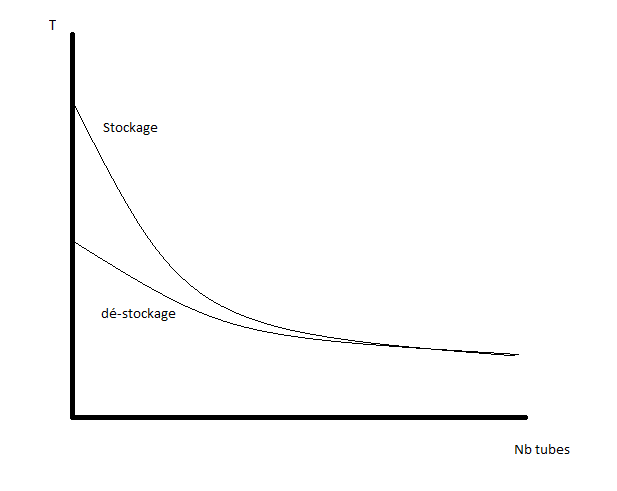
\includegraphics[scale=0.4]{PHOTO/courbe1.png}
	\label{graph1}
\end{figure}

\begin{figure}[!h]
	\centering
	\caption{Cycle 2 : Profil de température dans l'échangeur}
	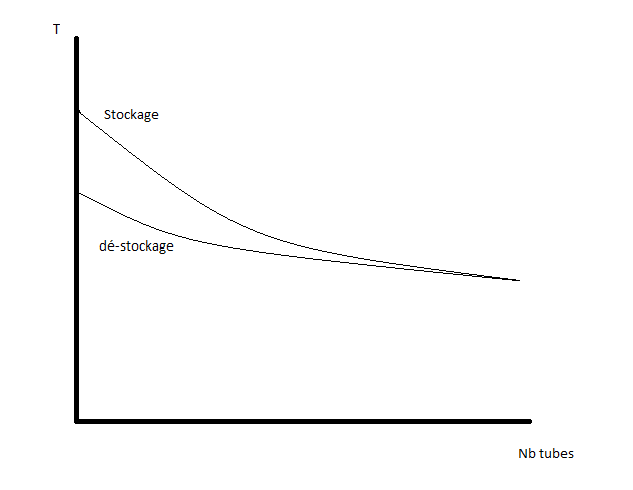
\includegraphics[scale=0.4]{PHOTO/courbe2.png}
	\label{graph2}
\end{figure}

\begin{figure}[!h]
	\centering
	\caption{Cycle nominal : Profil de température dans l'échangeur}
	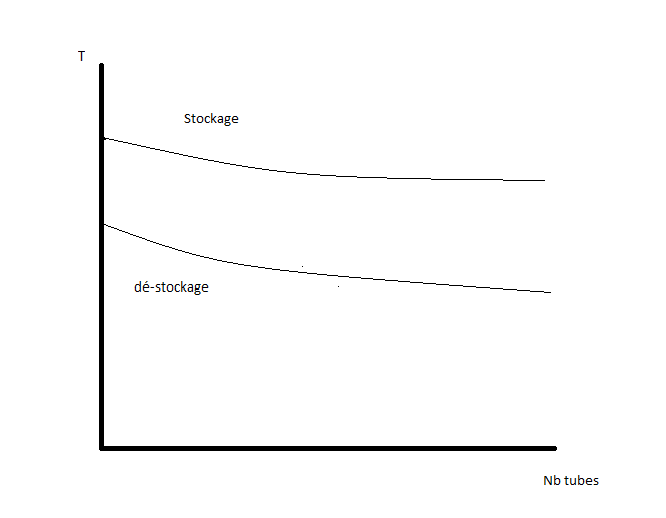
\includegraphics[scale=0.4]{PHOTO/courbe3.png}
	\label{graph3}
\end{figure}

\newpage

 Ce qui est essentiel de comprendre dans ces graphiques, c'est que nous avons un régime nominal qui se met en place au cour des stockages. Par conséquent, notre dimensionnement doit être fait pour le régime nominal. Ce qui va nous conduire à crée une boucle supplémentaire qui sera décrit dans le paragraphe suivant. 
\newpage

Nous pouvons remarquer qu'en alternant le sens de l'air dans le stockage de chaleur, nous avons une mise en place et un profil de régime nominal différent. Si on alternait le sens de l'air sur chaque cycle de stockage, le profil de température obtenue aurait l'allure suivante : 


\begin{figure}[!h]
	\centering
	\caption{Cycle nominal : Profil de température dans l'échangeur avec alternance du sens de l'air}
	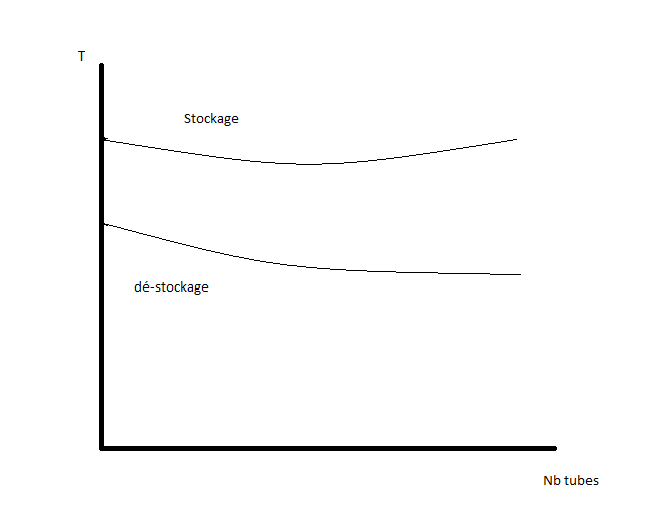
\includegraphics[scale=0.4]{PHOTO/courbe4.png}
	\label{graph4}
\end{figure}

Nous pourrions alors rechercher la meilleur configuration en alternant le sens du stockage et de-stockage. Nous nous limiterons ici au premier cas. 

\newpage
\section{Organigramme de la boucle}

\begin{figure}[!h]
	\centering
	\caption{Organigramme du dimensionnement en régime nominal}
	\includegraphics[scale=0.75]{PHOTO/organigramme_final.pdf}
	\label{graph3}
\end{figure}

\newpage
